\section{Solução da calibração}

O sensor a ser adquirido pelo projeto é o Faro Focus X330. Esse dispositivo
consiste em um \textit{laser scanner} e aquisita a distância percorrida pelo
feixe $laser$ emitido pelo sensor até o obstáculo mais próximo. A partir de um
espelho rotativo e um motor acoplado em sua base, o Focus X330 é capaz de
aquisitar pontos em $360^o$ na horizontal e $300^o$ na vertical. O modelo de
cada pá será, então, uma nuvem de pontos representando tridimensionalmente todas
as caracterísiticas necessárias.

As informações de distância recebidas pelos sensores descritos na seção
anterior podem ser armazenados como uma estrutura de dados chamada nuvem de
pontos, isto é, uma representação tridimensional do espaço cartesiano, na qual cada distância medida pelos
sensores a partir de sua origem representa uma coordenada x y z.
Entretanto, essa representação não é capaz de diferenciar, ou classificar, os
limites de cada objeto presente na cena, ou seja, não é possível determinar
\textit{a priori} qual conjunto de pontos pertence a cada elemento que se deseja
identificar para realizar a calibração.


A identificação de cada conjunto, ou \textit{cluster}, de pontos é importante
para que a posição e orientação de cada objeto de interesse seja determinada e,
assim a transformação do sistema de coordenadas entre cada objeto seja
calculada. Esse processo necessita, então, do estudo e implementação de
algoritmos para a análise da nuvem de pontos, identificação dos elementos
necessários, extração de suas respectivas posições e, finalmente, cálculo da
transformada entre as posições.

Dependendo das características de cada objeto a ser identificado e da
possibilidade de implementação de uma estrutura de apoio para facilitar a sua
identificação, podem ser utilizados diferentes métodos e estratégias de
identificação e localização, que serão exploradas a seguir.

\subsection{Reconhecimento do Robô}

O Robô é uma estrutura que a idenficação pode ser facilitada pelo uso de
padrões de fácil reconhecimento (como esferas e padrões de xadrez, figuras
\ref{fig::sphere_rec} e \ref{fig::checkerboard_rec} ), pois a
introdução de alterações na base do robô podem ser realizadas de maneira
estruturada e controlad, na etapa de construção do sistema, assegurando assim
uma calibração entre o posicionamento dos marcadores e o manipulador.


\begin{figure}[h!]
   \centering
   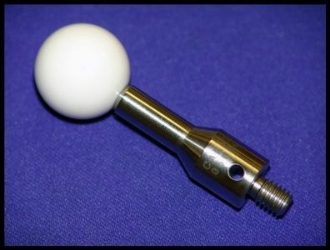
\includegraphics[width=0.95\columnwidth]{figs/calibracao/sphere_rec}
   \caption{Exemplo de esfera utilizada para reconhecimento. Fonte:
   http://shop.talwin.net/}
   \label{fig::sphere_rec}
\end{figure}



\begin{figure}[h!]
   \centering
   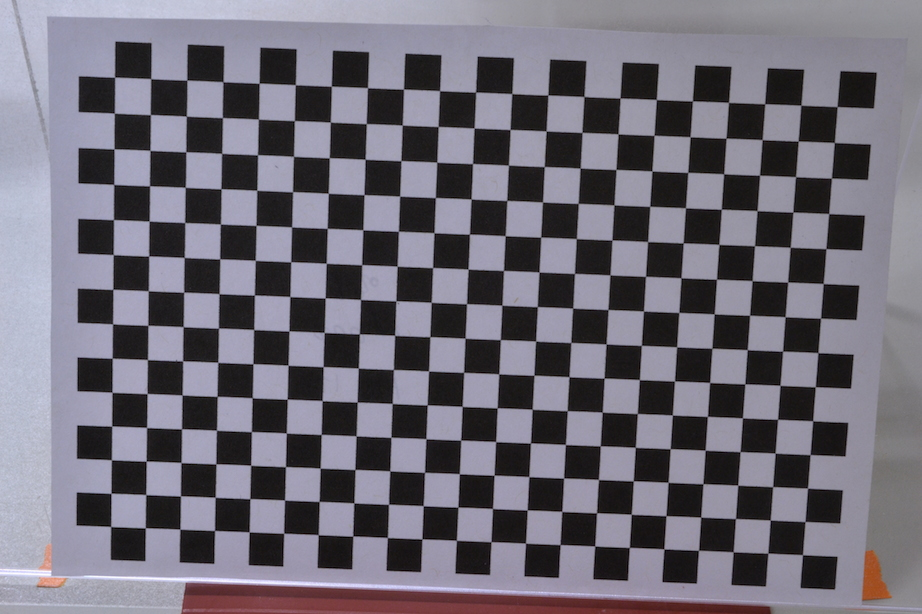
\includegraphics[width=0.95\columnwidth]{figs/calibracao/checkerboard_rec}
   \caption{Exemplo de padrão de xadrez utilizado para renhecimento.\\ Fonte:
   http://stereomorph.blogspot.com.br/}
   \label{fig::checkerboard_rec}
\end{figure}


Devido a baixa iluminação ambiente dentro do circuito hidráulico, a opção
mais simples é o uso de nuvem de pontos sem identificação de cor. Ou seja, o
reconhecimento se dará apenas pelo formato. Isso restringe o uso de padrões de
xadrez e o foco se voltará, então, para o uso de formatos geométricos. Em
especial o mais simples objeto de três dimensões: a esfera.

O reconhecimento de formas geométricas simples em três dimensões é um assunto
já razoavelmente explorado na literatura. Dentre eles pode-se destacar 2
métodos: RANSAC e Hough Transform.

\paragraph{RANSAC}
O método RANSAC (acrônimo para ``RANdom SAmple Consensus", \textit{consenso por
amostragem aleatória} em tradução livre) é um método iterativo que tem como
premissa a presença de \textit{outliers} (elementos fora do corpo principal) na
amostra e objetiva a identificação dos parâmetros matemáticos que descrevem o
objeto geométrico em questão \cite{ransac}. É o método
disponível na amplamente utilizada biblioteca de processamento de nuvem de pontos ``PCL''. 

%TODO REESCREVER
%********************************
Esse método consiste na seleção aleatória de pontos para serem considerados como
partes integrantes do corpo principal (no caso, uma esfera), a partir desses os
parâmetros da esfera são calculados (comumente, os valores x, y e z do centro
da esfera e seu raio). Então os demais pontos são julgados como fazendo parte ou
não da esfera de acordo com esses parâmetros. O modelo é avaliado como bem estimado se uma quantidade razoável de pontos são considerados
como pertencentes à esfera. Se for visto como bem estimado, os parâmetros são
então reestimado levando em conta de todos os pontos que foram considerados como
pertencentes à esfera. O erro do modelo é inferido a partir dos pontos que foram
considerados como fazendo parte da esfera e uma esfera reconstruída pelos
parâmetros calculados. O processo então é repetido um número artrário de vezes,
e se mantém armazenado o modelo que obteve menor erro.
%**************************************

Um dos principais pontos negativos do RANSAC é que ele tem como premissa a
presença de apenas um corpo principal, ou seja, apenas uma esfera. Isso implica
em um tratamento especial quando temos mais de uma esfera no ambiente.

\begin{figure}[h!]
   \centering
   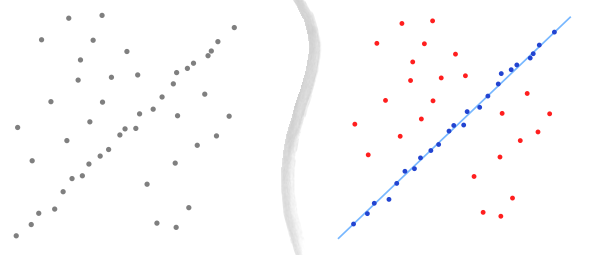
\includegraphics[width=0.95\columnwidth]{figs/calibracao/ransac}
   \caption{Exemplo de reconhecimento de uma linha em 2 dimensões usando
   RANSAC. (Fonte: \cite{ransac})}
   \label{fig::ransac}
\end{figure}
 
 \paragraph{Transformada de Hough 3D}
Anos de pesquisa em reconhecimento de objetos geométricos de duas dimensões
levaram ao desenvolvimento e aprimoramento de técnicas basedas em ``Transformada
de Hough''. Essas técnicas tem sido recentemente adaptadas para o universo de
três dimensões (ver \cite{hough2014}) e adequadamente chamadas de Transformada
de Hough 3D.

O método consiste em tranformar cada ponto do espaço 3D em uma variedade
mergulhada no espaço quadridimensional dos parâmetros da esfera ( x, y e z do
centro mais r do raio). A variedade se identifica com todas as possiveis esferas
que contém aquele ponto. O espaço de parâmetros é então restrito dentro de
certos limites e quantizado por razões de implementação (os recursos
computacionais são finitos). É definido então um acumulador, basicamente uma
função que conta quantas variedade interceptam determinada região discretizada
do espaço de parâmetros. Um algorítmo de reconhecimento de picos é aplicado
sobre o espaço de parâmetros (com as varidade já mergulhadas nele) para detectar
qual o conjunto de parâmetros que está melhor descrevendo um maior número de
pontos. O algorítmo pode ser utilizado para reconhecer mais de um pico e, assim,
identificar a presença de mais de uma esfera na nuvem de pontos (exemplo na
figura \ref{fig::hough}).

A dificuldade no uso do método é seu custo computacional, mas existem soluções
que exploram amostragens estatísticas para reduzir esse esforço.

\begin{figure}[h!]
   \centering
   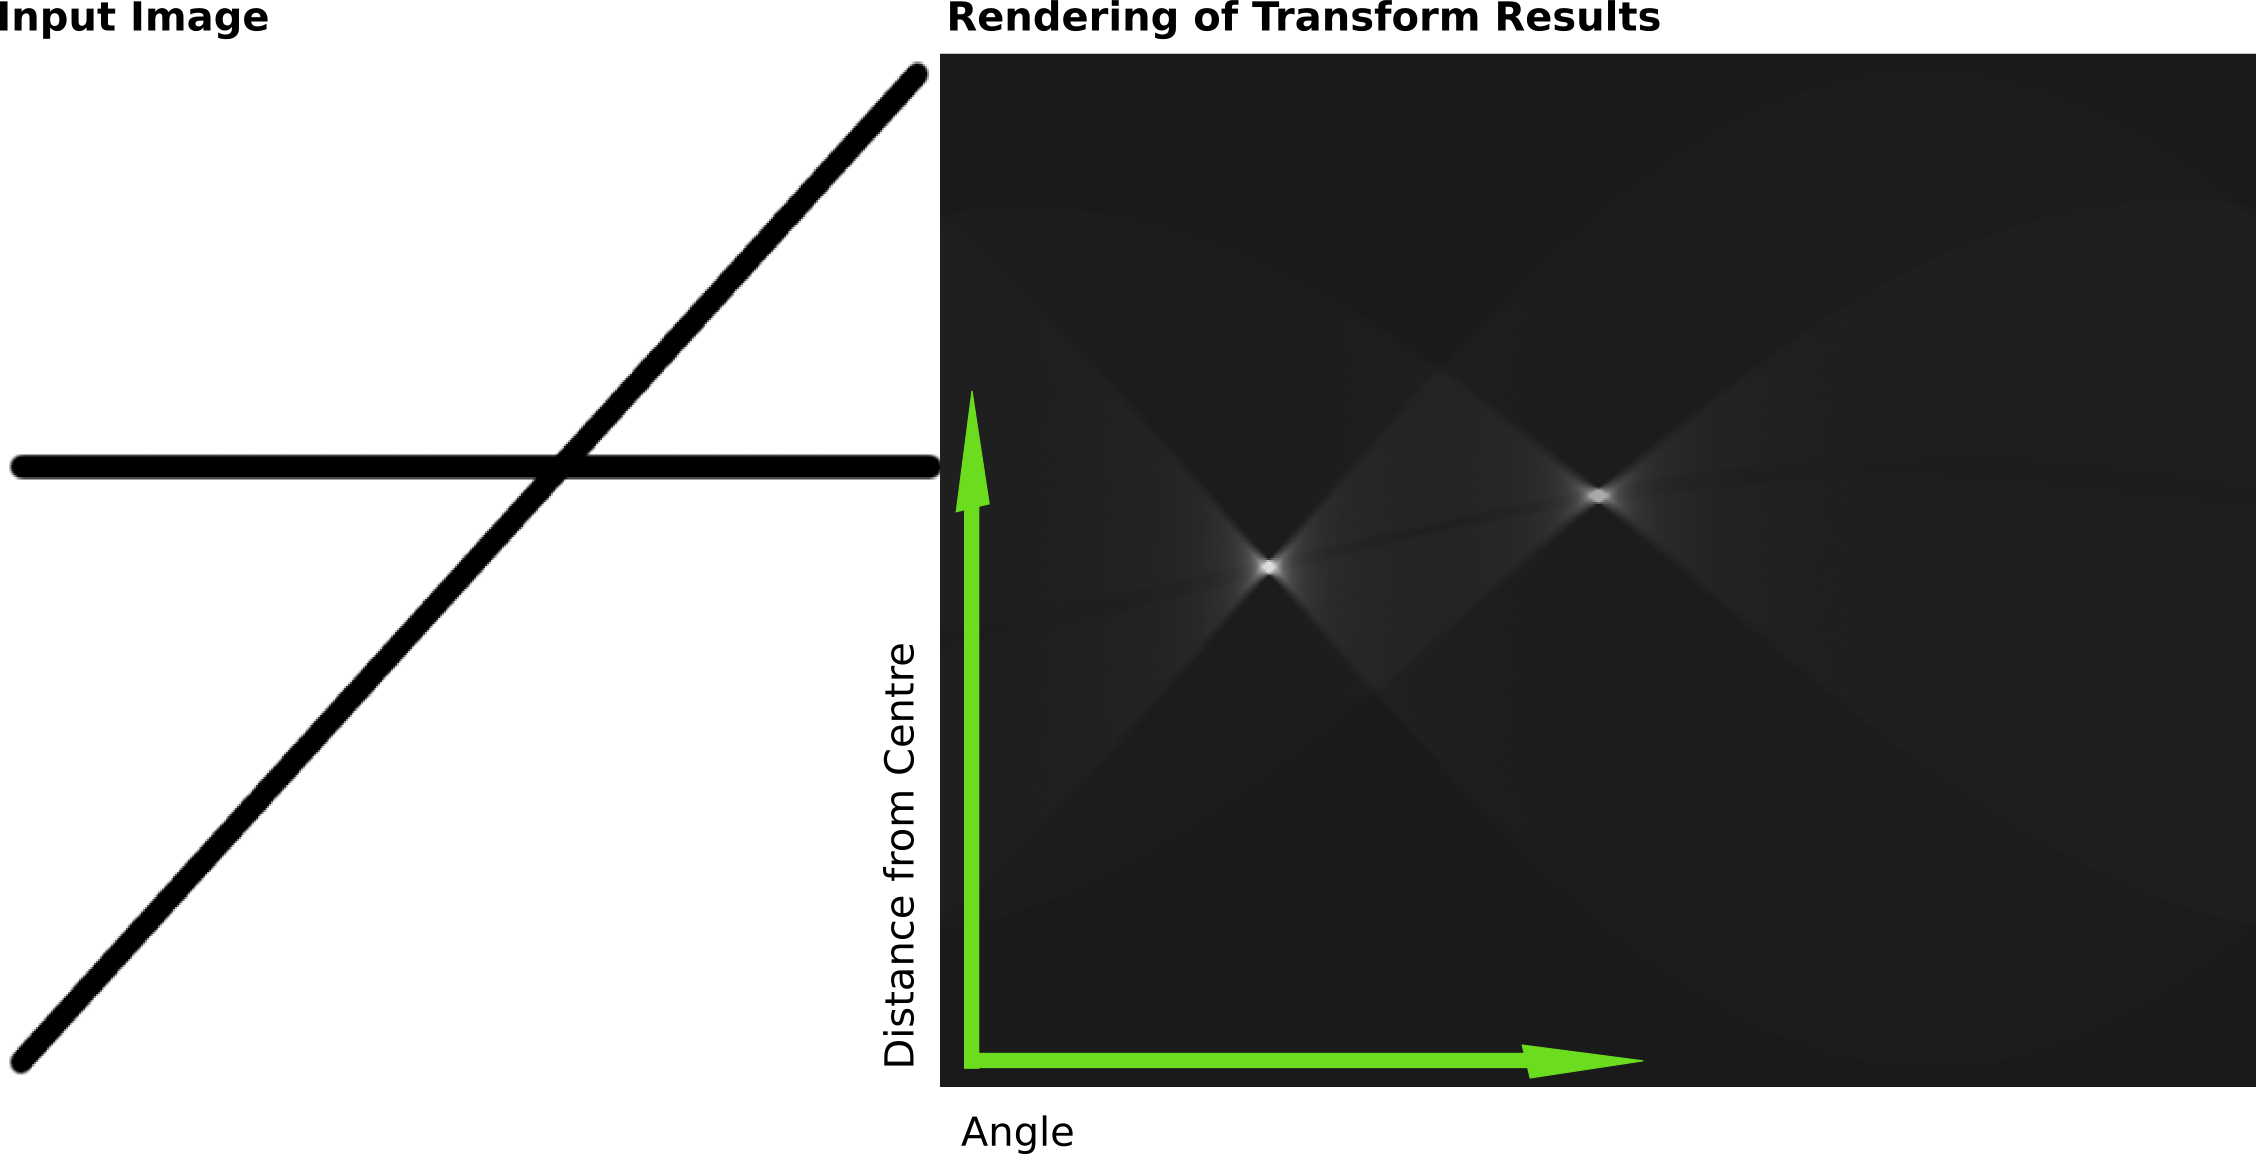
\includegraphics[width=0.95\columnwidth]{figs/calibracao/hough}
   \caption{Exemplo de reconhecimento de duas linhas em 2 dimensões usando
   Transformada de Hough. Na esquerda estão pontos que compõem as duas retas, na
   direita uma sobreposição das variedades referentes a cada ponto das retas
   (mergulhadas em um espaço paramétrico bidimensional). Os pontos mais
   brilhantes refletem os picos referentes aos parâmetros que melhor descrevem as duas retas. (Fonte: 
   \url{https://en.wikipedia.org/wiki/Hough_transform})}
   \label{fig::hough}
\end{figure}

Tendo conhecimento da posição de quatro esferas, pelo uso de um dos métodos
descritos acima, é possivel identificar unicamente a posição de um corpo preso
rigidamente ao conjunto de esferas. Em outras palavras, consegue-se a
transformada entre origem do sistema de coordenadas (tipicamente no sensor) e o robô. Para descobrir a trasnformada entre o robô e a pá (posição relativa entre eles) falta identificar a
transformada entre a origem e a pá, esse caso será explorado na próxima seção a
seguir.


\subsection{Calibração da pá}

Para a identificação e localização das pás das turbinas não é possível a
utilização de nenhum artifício de apoio que facilite o processamento da nuvem de
pontos, pois a instalação de qualquer um desses aparatos não pode ter precisão
garantida nas operações de campo. Uma instalação de um elemento de apoio em
pontos precisos da pá necessitaria também de calibração para cada utilização, retirando assim
o propósito do método. 

Portanto, para a localização das pás da turbina é
necessário explorar as características espaciais intrínsecas à superfície do
próprio objeto e identificá-las na nuvem de pontos do ambiente. O objetivo
principal nessa etapa do processo é, então, identificar um conjunto mínimo de
características do objeto que o represente unicamente com um baixo grau
de ambiguidade e sem exigir um esforço computacional elevado.

A escolha do tipo de característica a se usar é uma decisão fundamental para a
eficiência do processo e tem sido alvo de estudos na literatura para a análise
e reconhecimento de imagens 2D, como imagens RGB de câmeras e mais recentemente
também para imagens 3D. 

Uma boa representação de \textit{point feature} deve ser capaz de capturar as
mesmas características locais da superfície na presença de:

\begin{itemize}
  \item \textbf{Transformadas} -  rotações e translações 3D nos dados não devem
  influenciar a estimação dos descriptors;
  \item \textbf{Variações na densidade de amostragem} - em princípio, uma de
  superfície amostrada mais ou menos densamente deve ter a mesma assinatura característica do vetor
  \item \textbf{Ruído}
\end{itemize}

O reconhecimento de objetos em aplicações robóticas também vem recebido
grande atenção, principamente com o crescimento da robótica móvel e em ambientes
não estruturados, onde é necessário identificar e localizar os objetos a serem
manipulados em cada tarefa. O problema é enfrentado basicamente utilizando-se
duas abordagens: analisar os dados 3D ou realizar algum tipo de processamento e
projeção para se trabalhar com imagens 2D e utilizar as técnicas mais maduras
desse tipo de imagem.


Nesta última categoria, a técnica
mais usada consiste em converter as informações tridimensionais em \textit{Range
Images}, na qual é realizada uma projeção a partir de um ponto de vista (geralmente o do sensor) e utiliza escala
de cores ou cinza para representar a distância, ou seja, quanto mais escuro o
objeto na imagem, mais longe ele se encontra. É importante reassaltar que esse
tipo de método introduz perdas de informação ao se realizar projeções e é
sensível à escolha do ponto de vista escolhido. 

A escolha do descritor a ser
utilizado depende da aplicação e deve ser estudada a melhor opção para a nossa
solução, assim que tivermos dados aquisitados pelo sensor. Aplicações
semelhantes envolvendo identificação de objetos no ambiente tridimensional, mas
sem localizá-los, e utilizando diferentes descritores podem ser encotradas em
\cite{Bayramoglu2010,Hetzel2001,Chen2007}. Uma comparação dos descritores
utilizados para reconhecimento de objetos 2D e 3D pode ser encontrado em \cite{Zaharia2004, Weber2014}.

Após o reconhecimento do objeto, é necessário identificar a sua posição.
Em \cite{Steder2009}, o alinhamento é realizado utilizando-se a própria
\textit{Range Image} e a informação de profundidade presente na mesma. Por outro
lado, em \cite{Nuchter2005} a região onde o objeto identificado está presente é
selecionada e, por meio de \textit{raycasting} o conjunto de pontos da nuvem
pertecentes à região identificada na \textit{Range Image} é reprojetado. Após
essa segmentação, é utilizado um algoritmo de alinhamento como o ICP. 

%TODO encaixar texto

O formato original da pá do rotor é fixo para cara cada turbina, ou seja, uma
vez que definida em qual turbina será realizada a manutenção, é possível
fornecer \textit{a priori} qual tipo de pá será metalizada e suas
características. Essa característica possibilita descartar a necessidade de comparação e busca de
diversos modelos, reduzindo assim a complexidade computacional final do
algoritmo. Portanto, é possível armazenar uma representação de diferentes pás e
fornecer, como entrada do sistema, o modelo correto de acordo com o tipo de turbina que
está sendo inspecionada. O processo final consiste, então, no correto
posicionamento e alinhamento entre o modelo armazenado e a instância real do
objeto, ou mais especificamente a pá.

Os desenhos técnicos das pás, não fornecem informações suficientes
sobre o seu perfil hidráulico e, para fins práticos, os modelos serão adquiridos
a partir da inspeção \textit{in situ} de uma turbina em condições de conservação
que não apresente danos. Esse procedimento necessita ser realizado apenas uma
vez para cada modelo. Como especificado em \cite{EMMA DETAIL}, %TODO citar emma
% detail.
o sensor a ser adquirido pelo projeto é o Faro Focus X330. Esse dispositivo
consiste em um \textit{laser scanner} e aquisita a distância percorrida pelo
feixe $laser$ emitido pelo sensor até o obstáculo mais próximo. A partir de um
espelho rotativo e um motor acoplado em sua base, o Focus X330 é capaz de
aquisitar pontos em $360^o$ na horizontal e $300^o$ na vertical. O modelo de
cada pá será, então, uma nuvem de pontos representando tridimensionalmente todas
as caracterísiticas necessárias.

A partir da suposição que a pá se encontra dentro do campo de visão do sensor
$laser$, determinar a posição da pá consiste em posicionar a nuvem de pontos do
modelo de forma que ocorra uma sobreposição entre os pontos do modelo e da cena
e ambos conjuntos de pontos tenham as mesmas características, ou seja,
representem o mesmo objeto. A técnica a ser utilizada é denominada
\textit{correspondence grouping}. 


\subsubsection{\textit{Correspondence Grouping}}
 
O método proposto por \cite{Tombari2010a}, se baseia na identificação de
\textit{features} ou características tridimensionais locais para pontos de
interesse e identificar um conjunto de correspondências entre o modelo 3D e o a
cena analisada, no caso da aplicação do projeto EMMA as corresponências entre a
o modelo da pá e a turbina. Uma \textit{feature} descreve as caracteristicas da
vizinhança de um ponto, fornecendo assim informações locais para cada ponto. 

Para reduzir os cálculos necessários, é possível realizar uma amostragem na
nuvem de pontos e computar os descritores de cada caracteŕistica apenas para
pontos de interesse, tanto no modelo quanto na cena. Uma vez que ambos os
conjuntos de descritores foi calculado, deve-se então determinar as
correspondências entre os dois conjuntos. Pode-se utilizar, por exemplo, a
distância euclidiana entre os seus descritores correspondentes como medida
limite. Cada correspondência é uma evidência que o modelo se encontra na cena e
um acumulador é responsável por contabilizar os votos e um objeto é detectado
caso haja um número suficiente de votos. É importante ressaltar mesmo sendo
robusta a oclusões e ambientes com muita densidade de objetos, devido à presença de
ruído, e a particularidades de cada aplicação, como densidade e resolução das
nuvem de pontos forncecidas pelo sensor e pelo modelo, é possível a detecção de
falsos positivos, ou mesmo a incapacidade de se detectar corretamente o objeto
em questão. Para se tratar esse problema é necessário o correto ajuste de
diversos parâmetros e também a implementação de uma forma eficiente de avaliação
das hipóteses encontradas pelo algoritmo. 


\section{Simulação de nuvem de Pontos}

Devido a grande complexidade logística e a necessidade de disponibilidade de
acesso seco a uma turbina, é indispensável a possibilidade da sintetização de
dados consistentes e que representem de maneira eficaz as caracteristícas que
serão encontradas no cenário real de operação. 

\subsection{Dados genéricos}

Para um primeiro contato com o funcionamento do método \textit{Correspondence
Grouping} foram utilizados dados genéricos disponíveis na literatura
\footnotemark \footnotetext{http://kos.informatik.uni-osnabrueck.de/3Dscans/}
e um modelo da pá gerado pelo sensor Faro Focus X330 , durante a viagem de campo
à Usina Hidrelética de Jirau para o teste de viabilidade técnica desse sensor, foi
introduzido artificialmente na cena.

A figura \ref{fig::modelo_pa_faro} ilustra o modelo da pá em nuvem de pontos,
esse modelo é uma representação de $360^o$ da superfície da pá e foi aquisitado em
campo, sendo assim representa a real leitura final do sensor na aplicação do
algoritmo de calibração.

\begin{figure}[h!]
	\centering
	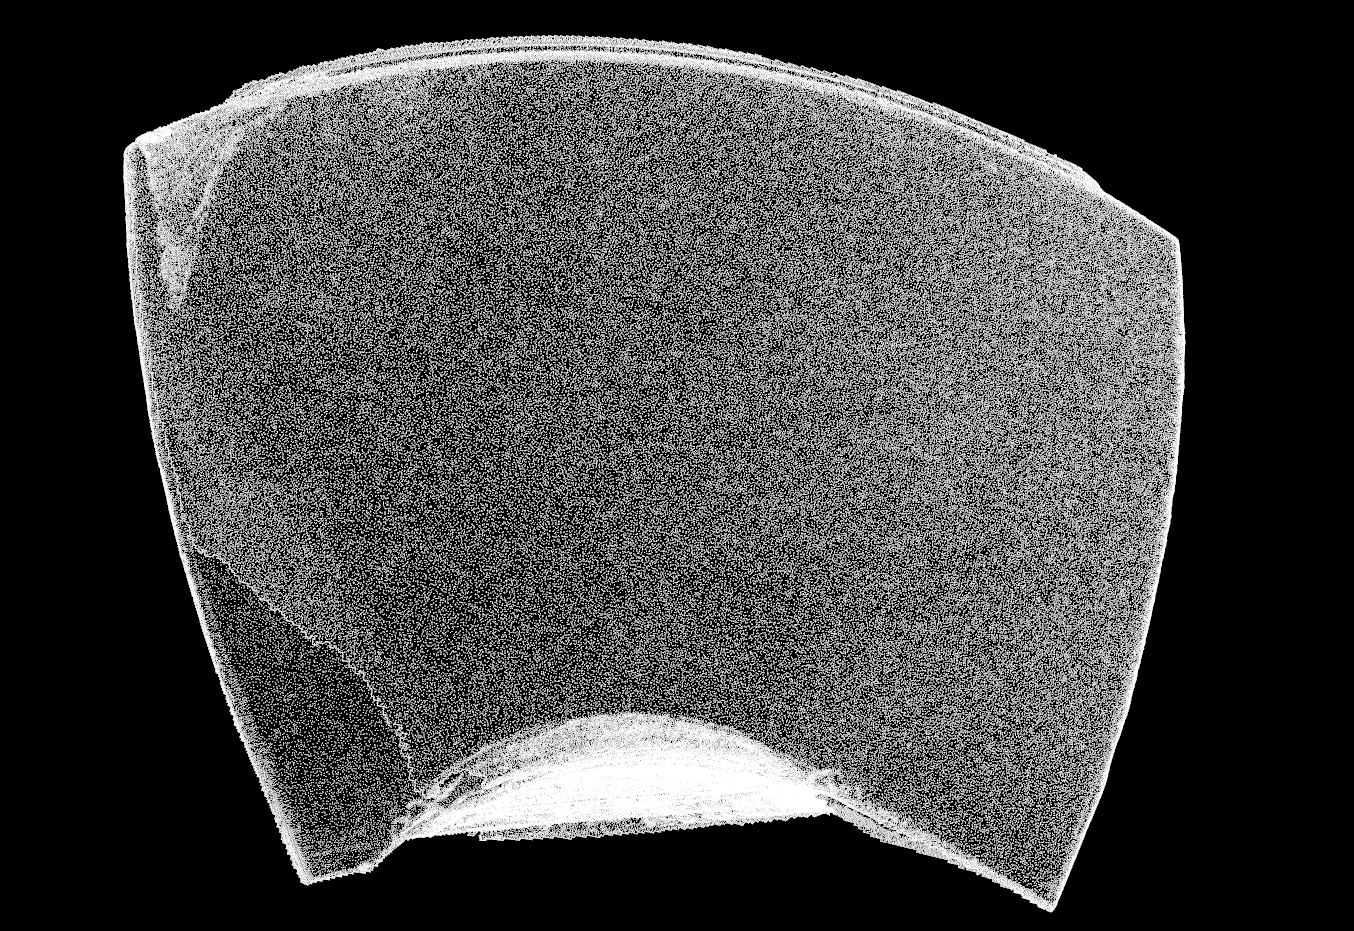
\includegraphics[width=0.9\columnwidth]{figs/calibracao/modelo_pa_faro}
	\caption{Nuvem de pontos da pá aquisitada pelo sensor Faro Focus X330.}
    \label{fig::modelo_pa_faro}
\end{figure}

A identificação da objeto na cena e a estimação da sua posição foi testada em
uma cena de um escritório, como pode ser visualizado na figura
\ref{fig::pa_cena_gen}. O modelo foi sobreposto em vermelho e não houve uma
discrepância visível entre a instância presente na cena e o modelo sobreposto. 
Mesmo com uma diferença de densidade de pontos presente em cada parte da nuvem
de pontos resultante (modelo é muito mais denso que a cena), foi possível
realizar a correta localização do modelo. O ajuste dos paramêtros de
subamostragem necessitaram de maior atenção nesse cenário. Vale ressaltar que o
algoritmo identificou corretamente uma cópia exata do modelo que foi introduzido
na cena, não há presença de ruídos ou oclusões no instância da pá presente na
cena.

\begin{figure}[h!]
	\centering
	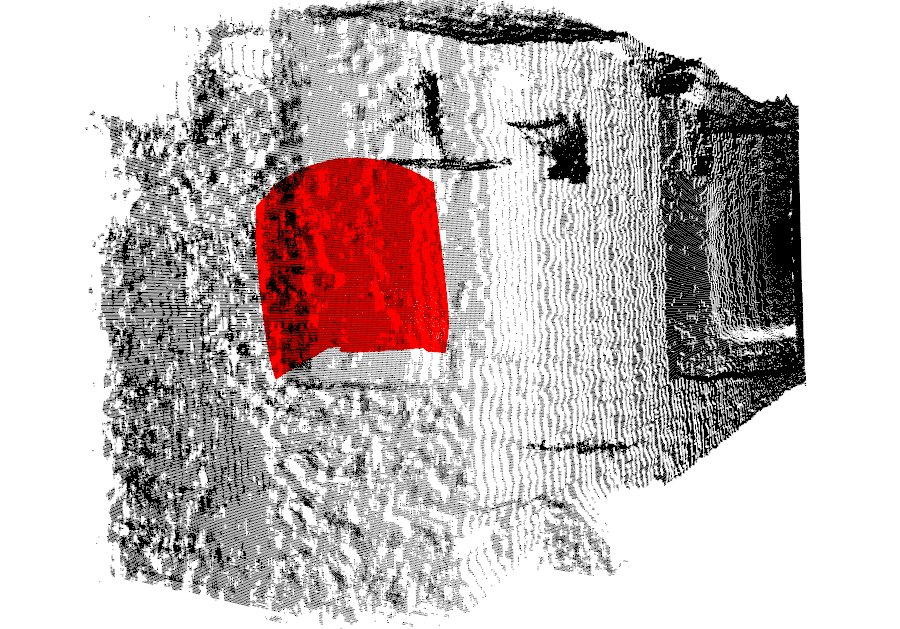
\includegraphics[width=0.9\columnwidth]{figs/calibracao/blade_office5}
	\caption{Exemplo de localização do modelo da pá em uma cena genérica.}
    \label{fig::pa_cena_gen}
\end{figure}

\subsection{Blensor}

A utilização de dados genéricos é útil para a implementação e testes do
algoritmo, entretanto não representa as condições reais que serão encontradas
durante o processo de metalização. A geometria da turbina, da pá, do manipulador
e também as oclusões geradas pelos elementos presentes necessitam ser simulados
para um perfeito ajuste do sistema. Para a simulação desses cenários, foi
utilizado a \textit{toolbox Blensor}\footnotemark
\footnotetext{http://www.blensor.org} baseada no \textit{software} de criação 3D
\textit{Blender}\footnotemark \footnotetext{http://www.blender.org}, o qual
permite a simulação da nuvem de pontos resultante de um sensor em um ambiente
tridimensional. Os objetos inseridos na cena são sólidos 3D, que podem ser
desenhados utilizando-se as ferramentas do próprio programa ou importados de
outros  em outros formatos suportados, como a partir do
Solidworks\textregistered por exemplo. A Figura \ref{fig::blensor_screen}
ilustra a utilização do software, assim como o modelo 3D da turbina importado. A
simulação leva em consideração a distância percorrida pelo pulso emitido, a
intensidade luminosa retornada ao sensor e o tempo decorrido durante o
sensoriamento \cite{Gschwandtner2011}, o que fornece uma melhor aproximação da
resposta do sensor para um ambiente simulado do que simplesmente a utilização de
uma técnica de \textit{raycast} pura.

\begin{figure}[h!]
	\centering
	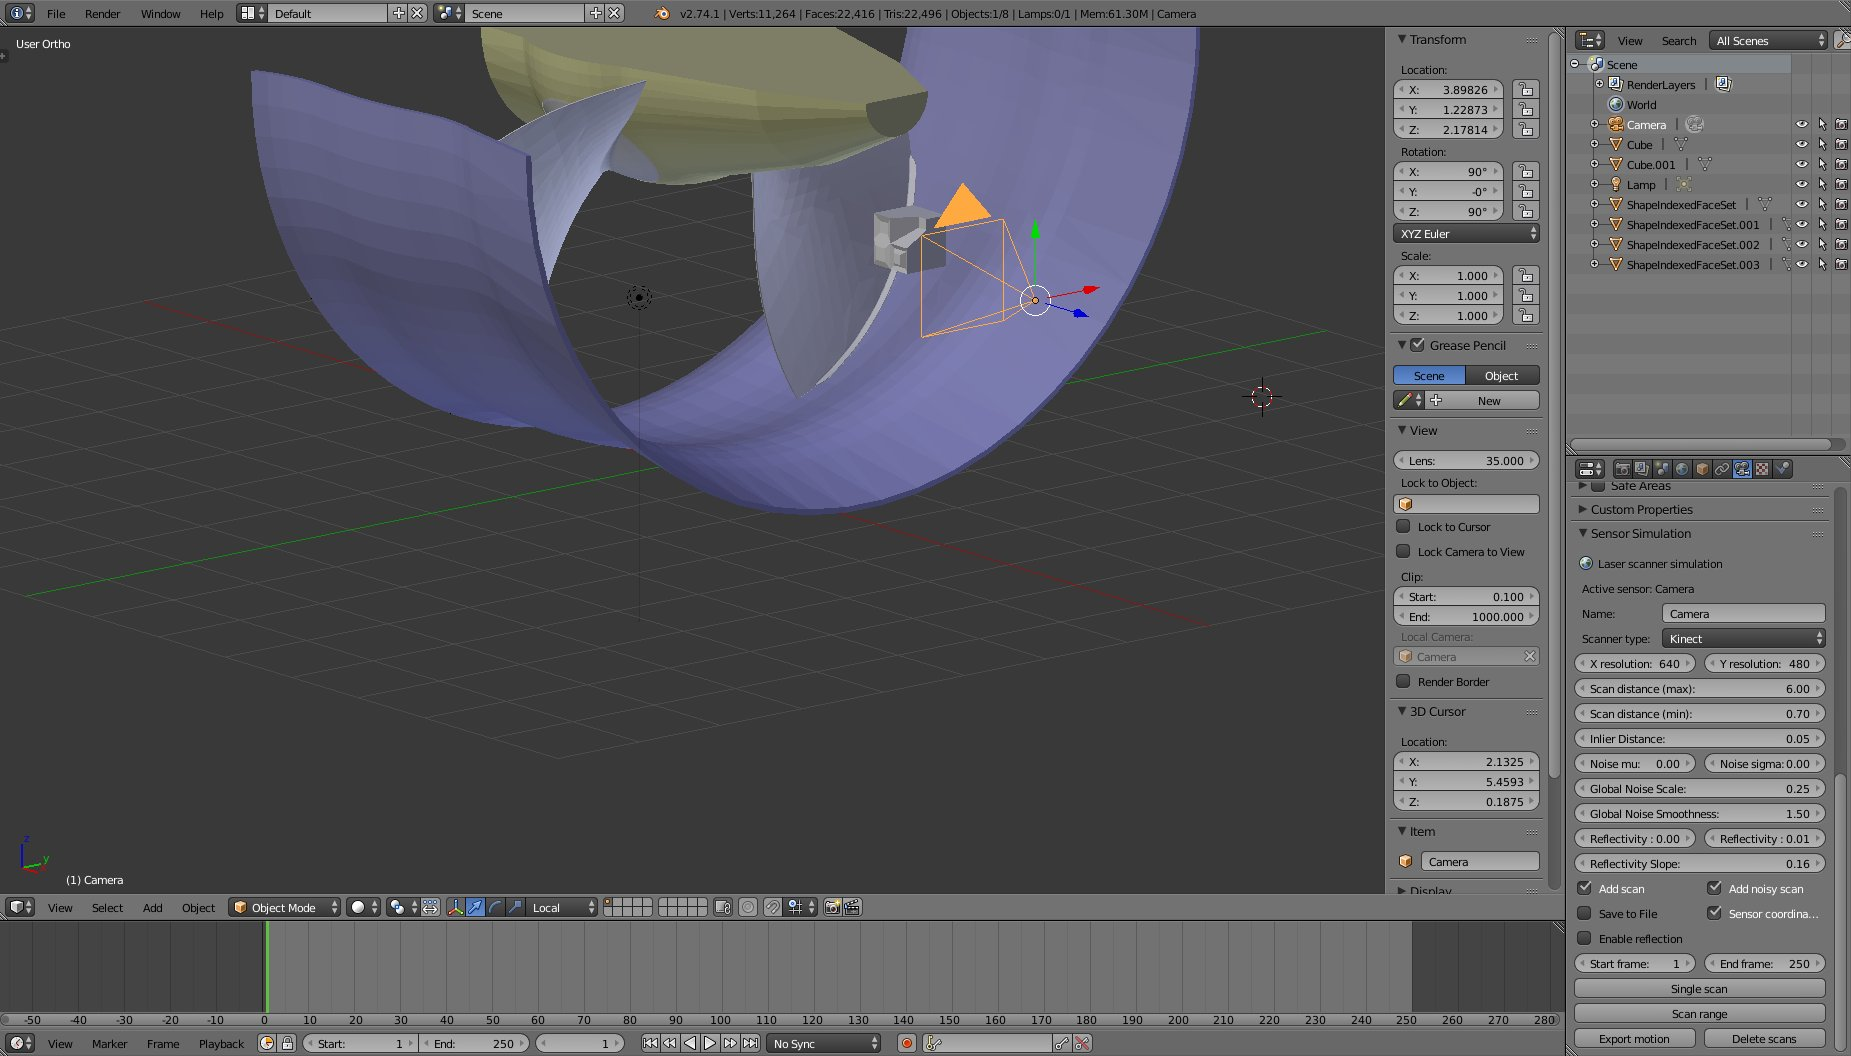
\includegraphics[width=0.9\columnwidth]{figs/calibracao/blensor_screen}
	\caption{Visualização do \textit{Blensor} com o modelo 3D da turbina
	importado.}
    \label{fig::blensor_screen}
\end{figure}

Dentro do ambiente de simulação, é possível a sintetização de dados provenientes
de diversos tipos de sensores laser, como um laserscanner 2D, o sensor
Velodyne e sensores do tipo Kinect. Os parâmetros de configuração
dos sensores também estão disponíveis para ajuste, assim como o nível de ruído. Sensores que não estão
nativamente disponíveis podem ser introduzidos. O sensor Faro Focus X330 não
pertence a lista de sensores previamente carregados pela ferramenta e teve que
ser implementado. As especificações técnicas utilizadas estão de acordo com as
fornecidas pelo fabricante, com exceção do ângulo de visão que foi reduzido para
diminuir o esforço computacional, sem perda de informação. A figura
\ref{fig::blensor_faro} ilustra a resposta simulada do sensor implementado
dentro do ambiente de simulação com a presença do modelo CAD da turbina.


 \begin{figure}[H]
	\centering
	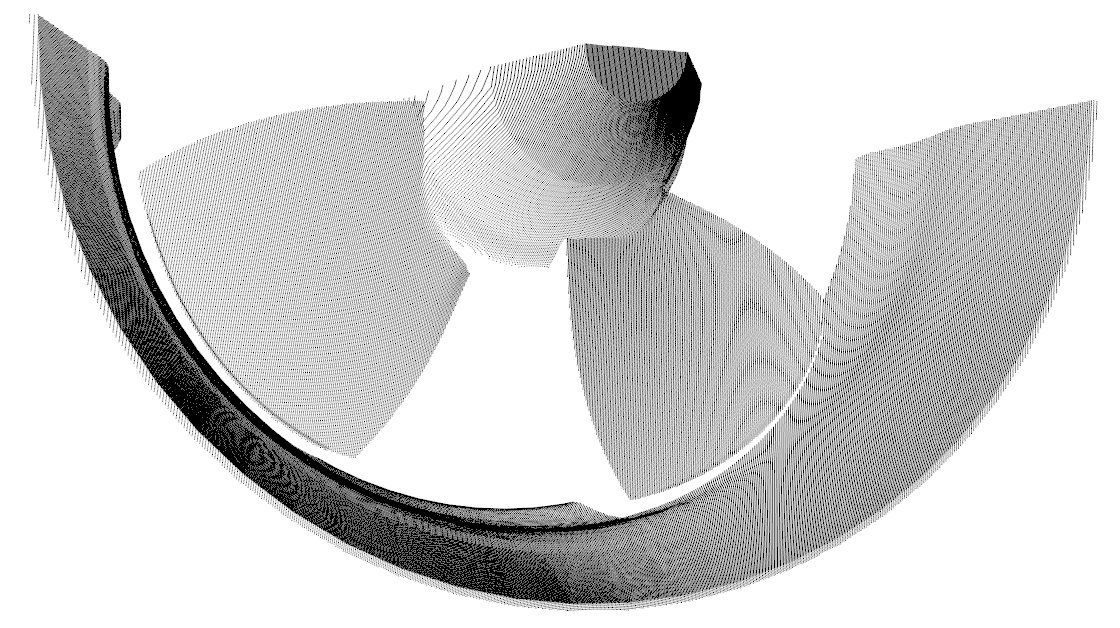
\includegraphics[width=0.9\columnwidth]{figs/calibracao/blensor_faro}
	\caption{Resposta simulada do sensor Faro Focus X330.}
    \label{fig::blensor_faro}
\end{figure}	


Caso seja disponibilizado uma descrição do perfil hidráulico da pá, é possível
também a geração de modelos sem a necessidade de uma inspeção prévia em uma
unidade geradora, na qual haja a presença de dados nas pás, para a aquisição de
dados sobre a turbina. A figura \ref{fig::modelo_pa} ilustra o ambiente de simulação e a
nuvem de pontos final para a criação de um modelo a partir de um arquivo
descritivo. 


\begin{figure}[h!]
	\centering
	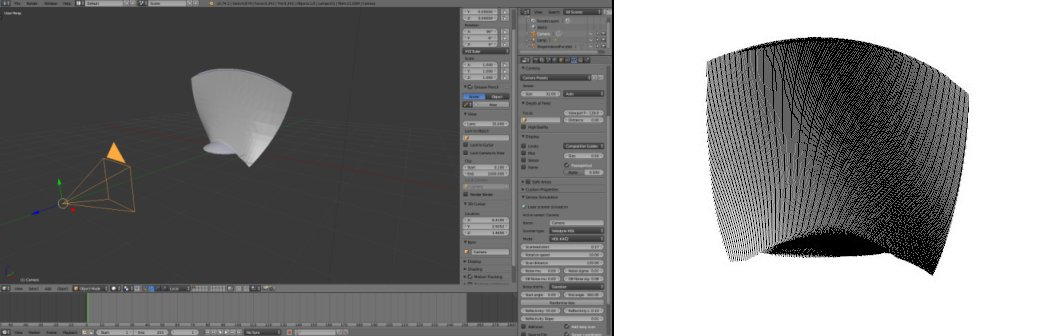
\includegraphics[width=0.9\columnwidth]{figs/calibracao/blensor_pa_sim}
	\caption{Criação de um sensor a partir de um arquivo descritivo da pá.}
    \label{fig::modelo_pa}
\end{figure}

Para representar corretamente as oclusões geradas pelo própria estrutura do
rotor e das pás, é necessário que as cenas sintetizadas a partir da ferramenta
tenham o sensor virtual posicionado em posições que representem os locais no
qual é possível a fixação real do equipamento dentro da UG. As oclusões geradas
pelo sistema de metalização também devem ser previstas e simuladas para um
perfeito ajuste do algoritmo, uma vez que o conjunto do robô e trilhos deve
estar previamente posicionado para que a calibração entre a pá e o efetuador do
manipulador seja realizada. Para isso, o modelo do manipulador MH12 foi
importado para dentro do ambiente de simulação, como ilustrado na figura
\ref{fig::model_mh12} e, em seguida, posicionado entre o sensor e a pá, para
servir de obstáculos para parte dos feixe laser que atingiriam a pá.


\begin{figure}[H]
	\centering
	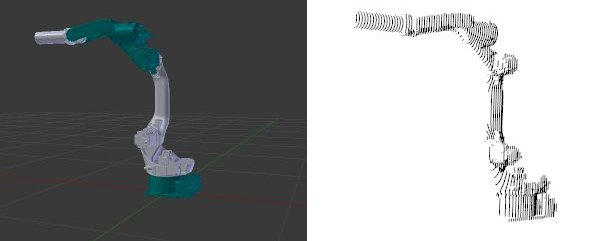
\includegraphics[width=0.9\columnwidth]{figs/calibracao/mh12_model}
	\caption{Visualização do \textit{Blensor} com o modelo 3D da turbina
	importado.}
    \label{fig::model_mh12}
\end{figure}

A Figura \ref{fig::sim_mh12}
ilustra a pá sendo corretamente identificada com a presença do manipulador entre
o sensor e a pá criando uma região de sombra. É possível observar o modelo que
está sendo comparado à cena na parte direita da figura e as linhas verdes
representam as correspondências encontradas entre os descritores do modelo da pá
e os encontrados na cena.

\begin{figure}[H]
	\centering
	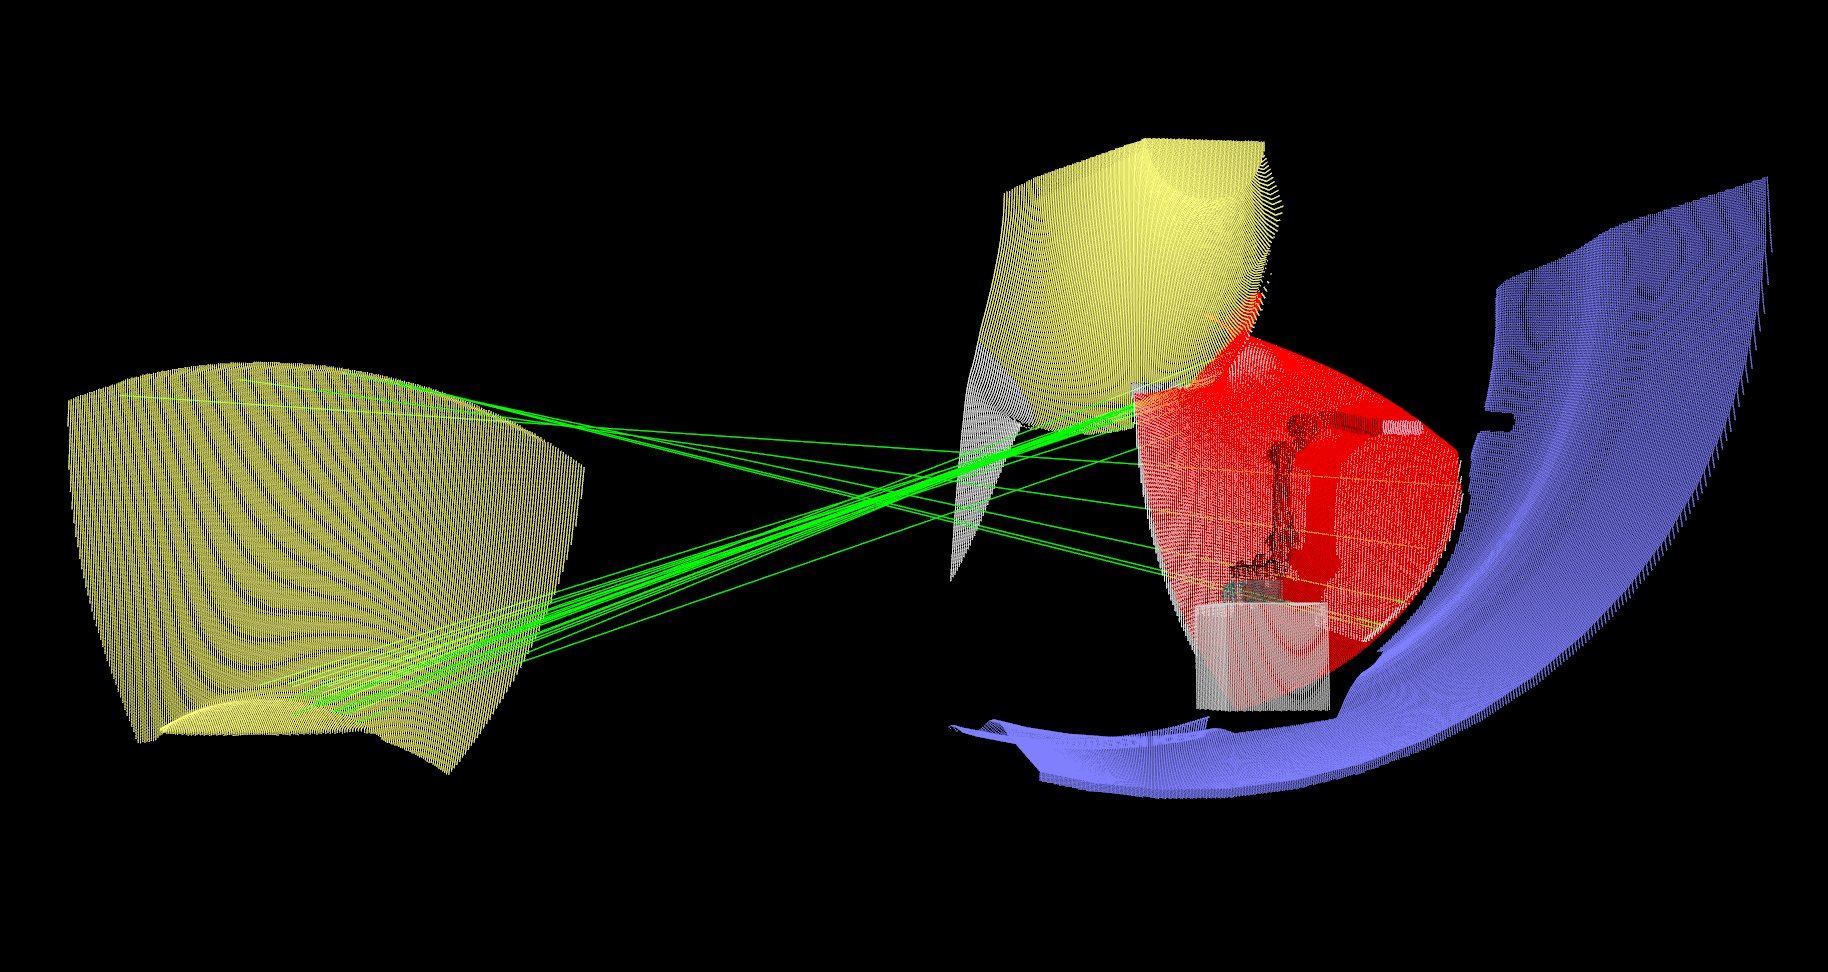
\includegraphics[width=0.9\columnwidth]{figs/calibracao/sim_mh12_sp}
	\caption{Resposta simulada do sensor Faro Focus X330.}
    \label{fig::sim_mh12}
\end{figure}	
